\chapter*{Curriculum Vitae}
\thispagestyle{empty}

% \begin{wrapfigure}{R}{3.5cm}
%     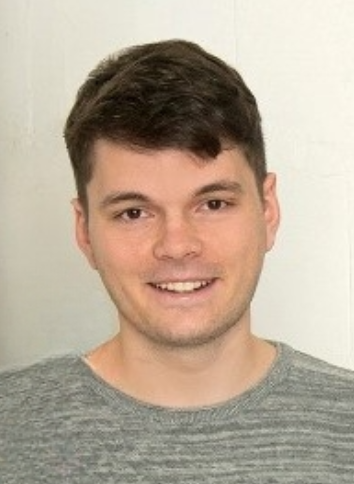
\includegraphics[width=3.5cm]{profile}
% \end{wrapfigure}

\markboth{Sebastian Hirt}{Sebastian Hirt} % falls der CV über 2 Seiten geht um einen "Running Header" zu haben

\flushright
% Code mit Bild:
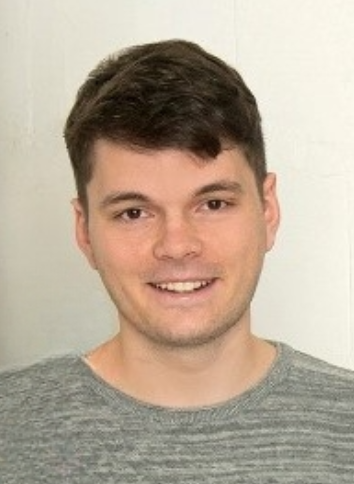
\includegraphics[scale=.3]{profile}
\vspace*{-5cm}
%Code ohne Bild:
%\vspace*{-1cm}{
\subsection*{Personal Data}
\flushleft
%\tabular-Umgebung
\normalsize
\begin{tabular}{lcl}
Address             & ~ & Moltkestraße 6\\
                    & ~ & 91054 Erlangen\\[5pt]
Email               & ~ & sebastian.hirt@fau.de\\[5pt]
Date of birth        & ~ & 26.07.1996\\
Nationality & ~ & german\\
\end{tabular} 

\nopagebreak
\subsection*{Education}
\begin{tabular}{lcl}
09/2006 - 07/2014     & ~~~ &  Werner-von-Siemens-Gymnasium, Weißenburg\\
10/2014 - 09/2020     & ~~~ &  Bachelor of Science\\
                      & ~~~ &  Friedrich-Alexander-Universität Erlangen-Nürnberg\\
10/2020 - 09/2023     & ~~~ &  Master of Science\\
                      & ~~~ &  Friedrich-Alexander-Universität Erlangen-Nürnberg\\
\end{tabular}

\vfill


Erlangen, \today \\*[20pt]\nopagebreak
\vspace{0.5cm}


\rule{5cm}{0.4pt}\\*\nopagebreak


Sebastian Hirt\\*\nopagebreak
